%%%%%%%%%%%%%%%%%%%%%%%%%%%%%%%%%%%%%%%%%%%%%%
%                insertmeeting
% 1) Title (something creative & funny?)
% 2) Date (MM/DD/YYYY)
% 3) Location (ex. Hagerty High School)
% 4) People/Committees Present 
% 5) Picture 
% 6) Start Time & Stop Time (ex. 12:30AM to 4:30PM)
%%%%%%%%%%%%%%%%%%%%%%%%%%%%%%%%%%%%%%%%%%%%%%
\insertmeeting 
	{Pipeline Problems} 
	{01/24/22} 
	{Hagerty High School}
	{Annika, Anouska, Clayton, Falon, James, Jensen, Nathan, Ritam, Rose, Samantha, Lilly}
	{Images/RobotPics/robot.jpg}
	{2:30 - 4:30}
	
\hhscommittee{Software}
\noindent\hfil\rule{\textwidth}{.4pt}\hfil
\subsubsection*{Goals}
\begin{itemize}
    \item Implement and test the OpenCV Pipeline to detect the Carousels

\end{itemize} 

\noindent\hfil\rule{\textwidth}{.4pt}\hfil

\subsubsection*{Accomplishments}
Last meeting we were able to complete preliminary work on an OpenCV Pipeline. Using a tool named GRIP from wpi Robotics to quickly test OpenCV pipelines. We decided on using an HSV Threshold to find blue, then erode and dilate the image before finding contours to achieve the best possible results. Luckily, GRIP included a feature that was able to generate code for the pipeline we made using the GUI. Today we were able to begin applying that pipeline to our testing code. After putting the code onto a Control Hub and attaching a webcam, we were able to display the results on the TV (Image attached). Surprisingly, the pipeline worked well. It was able to detect various blue-colored objects. However, it was detecting multiple objects and returning them all as objects. To solve this issue, we decided to calculate the height to width ratio for each contour, educatedly guessing that the carousel pole would have the largest ratio. After this change, our pipeline only returns one contour - the blue carousel. It seems to work well for multiple angles and far distances. Next meeting we will focus on implementing the same pipeline with a modified HSV threshold for the red side. 

\begin{figure}[ht]
\centering
\begin{minipage}[b]{.48\textwidth}
  \centering
  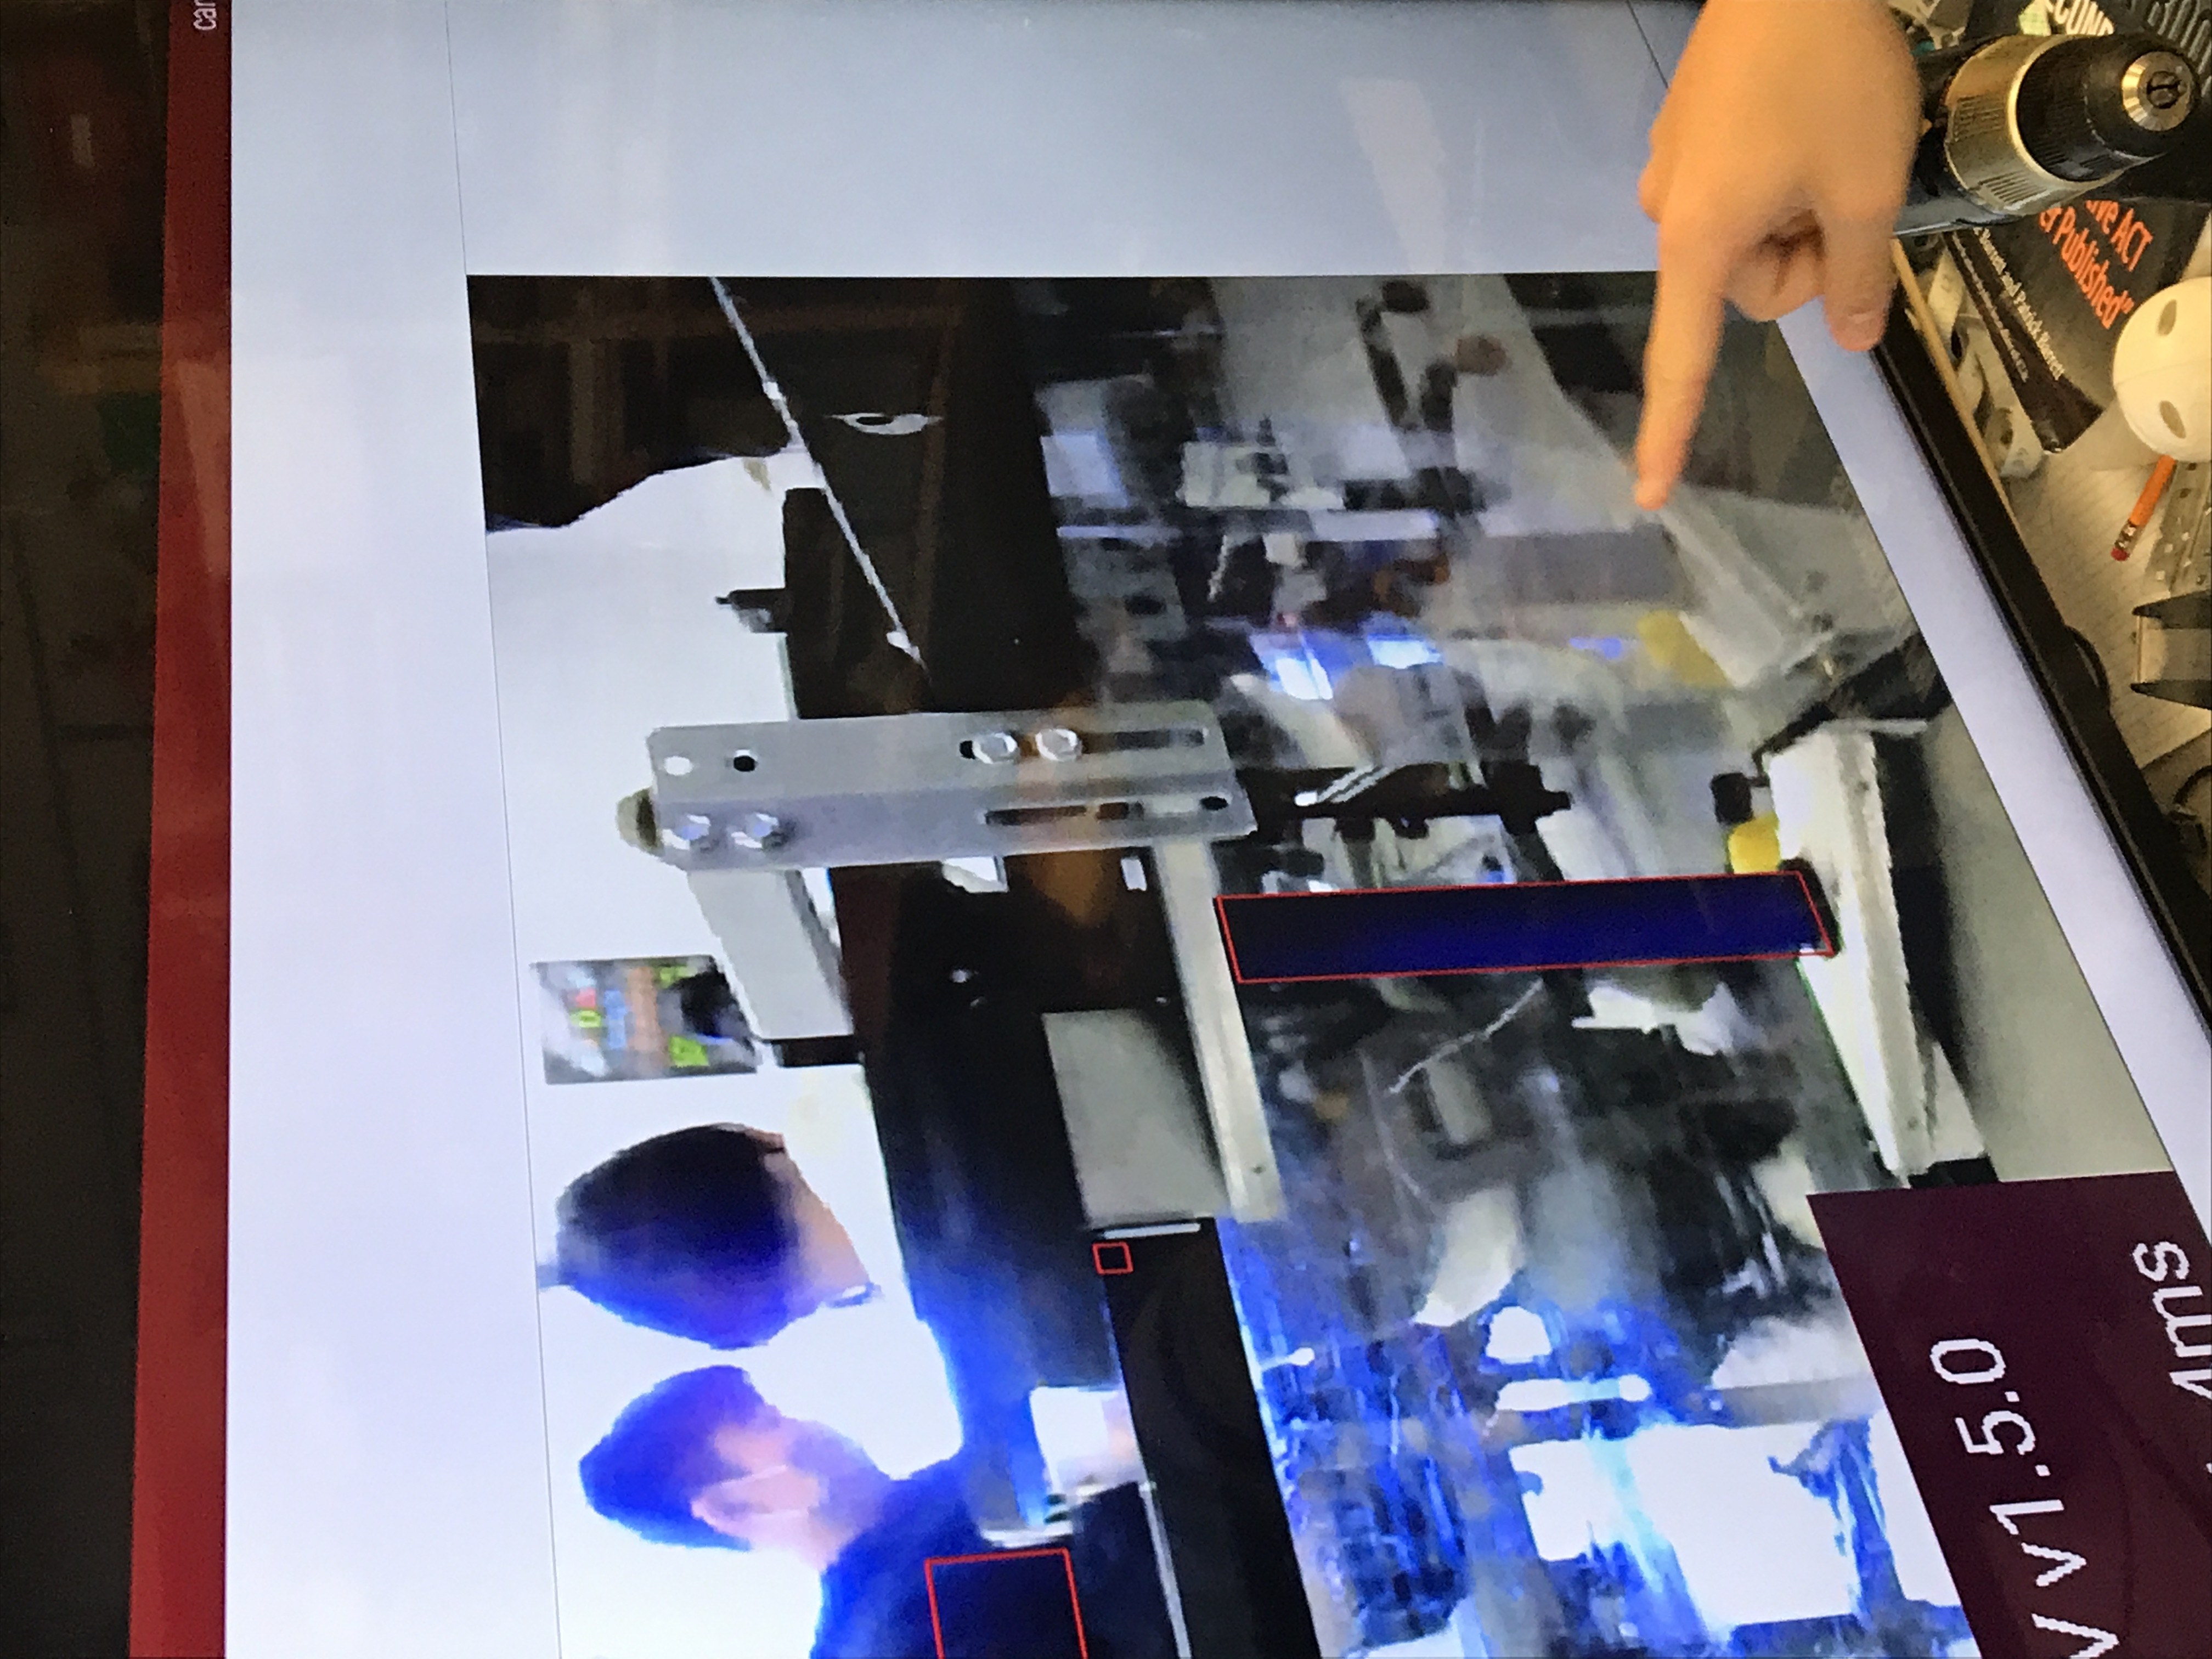
\includegraphics[width=0.95\textwidth]{Meetings/January/01-24-22/IMG_5646 - James Hu.JPG}
  \caption{Our pipeline in action}
  \label{fig:012422_1}
\end{minipage}%
\hfill%
\begin{minipage}[b]{.48\textwidth}
  \centering
  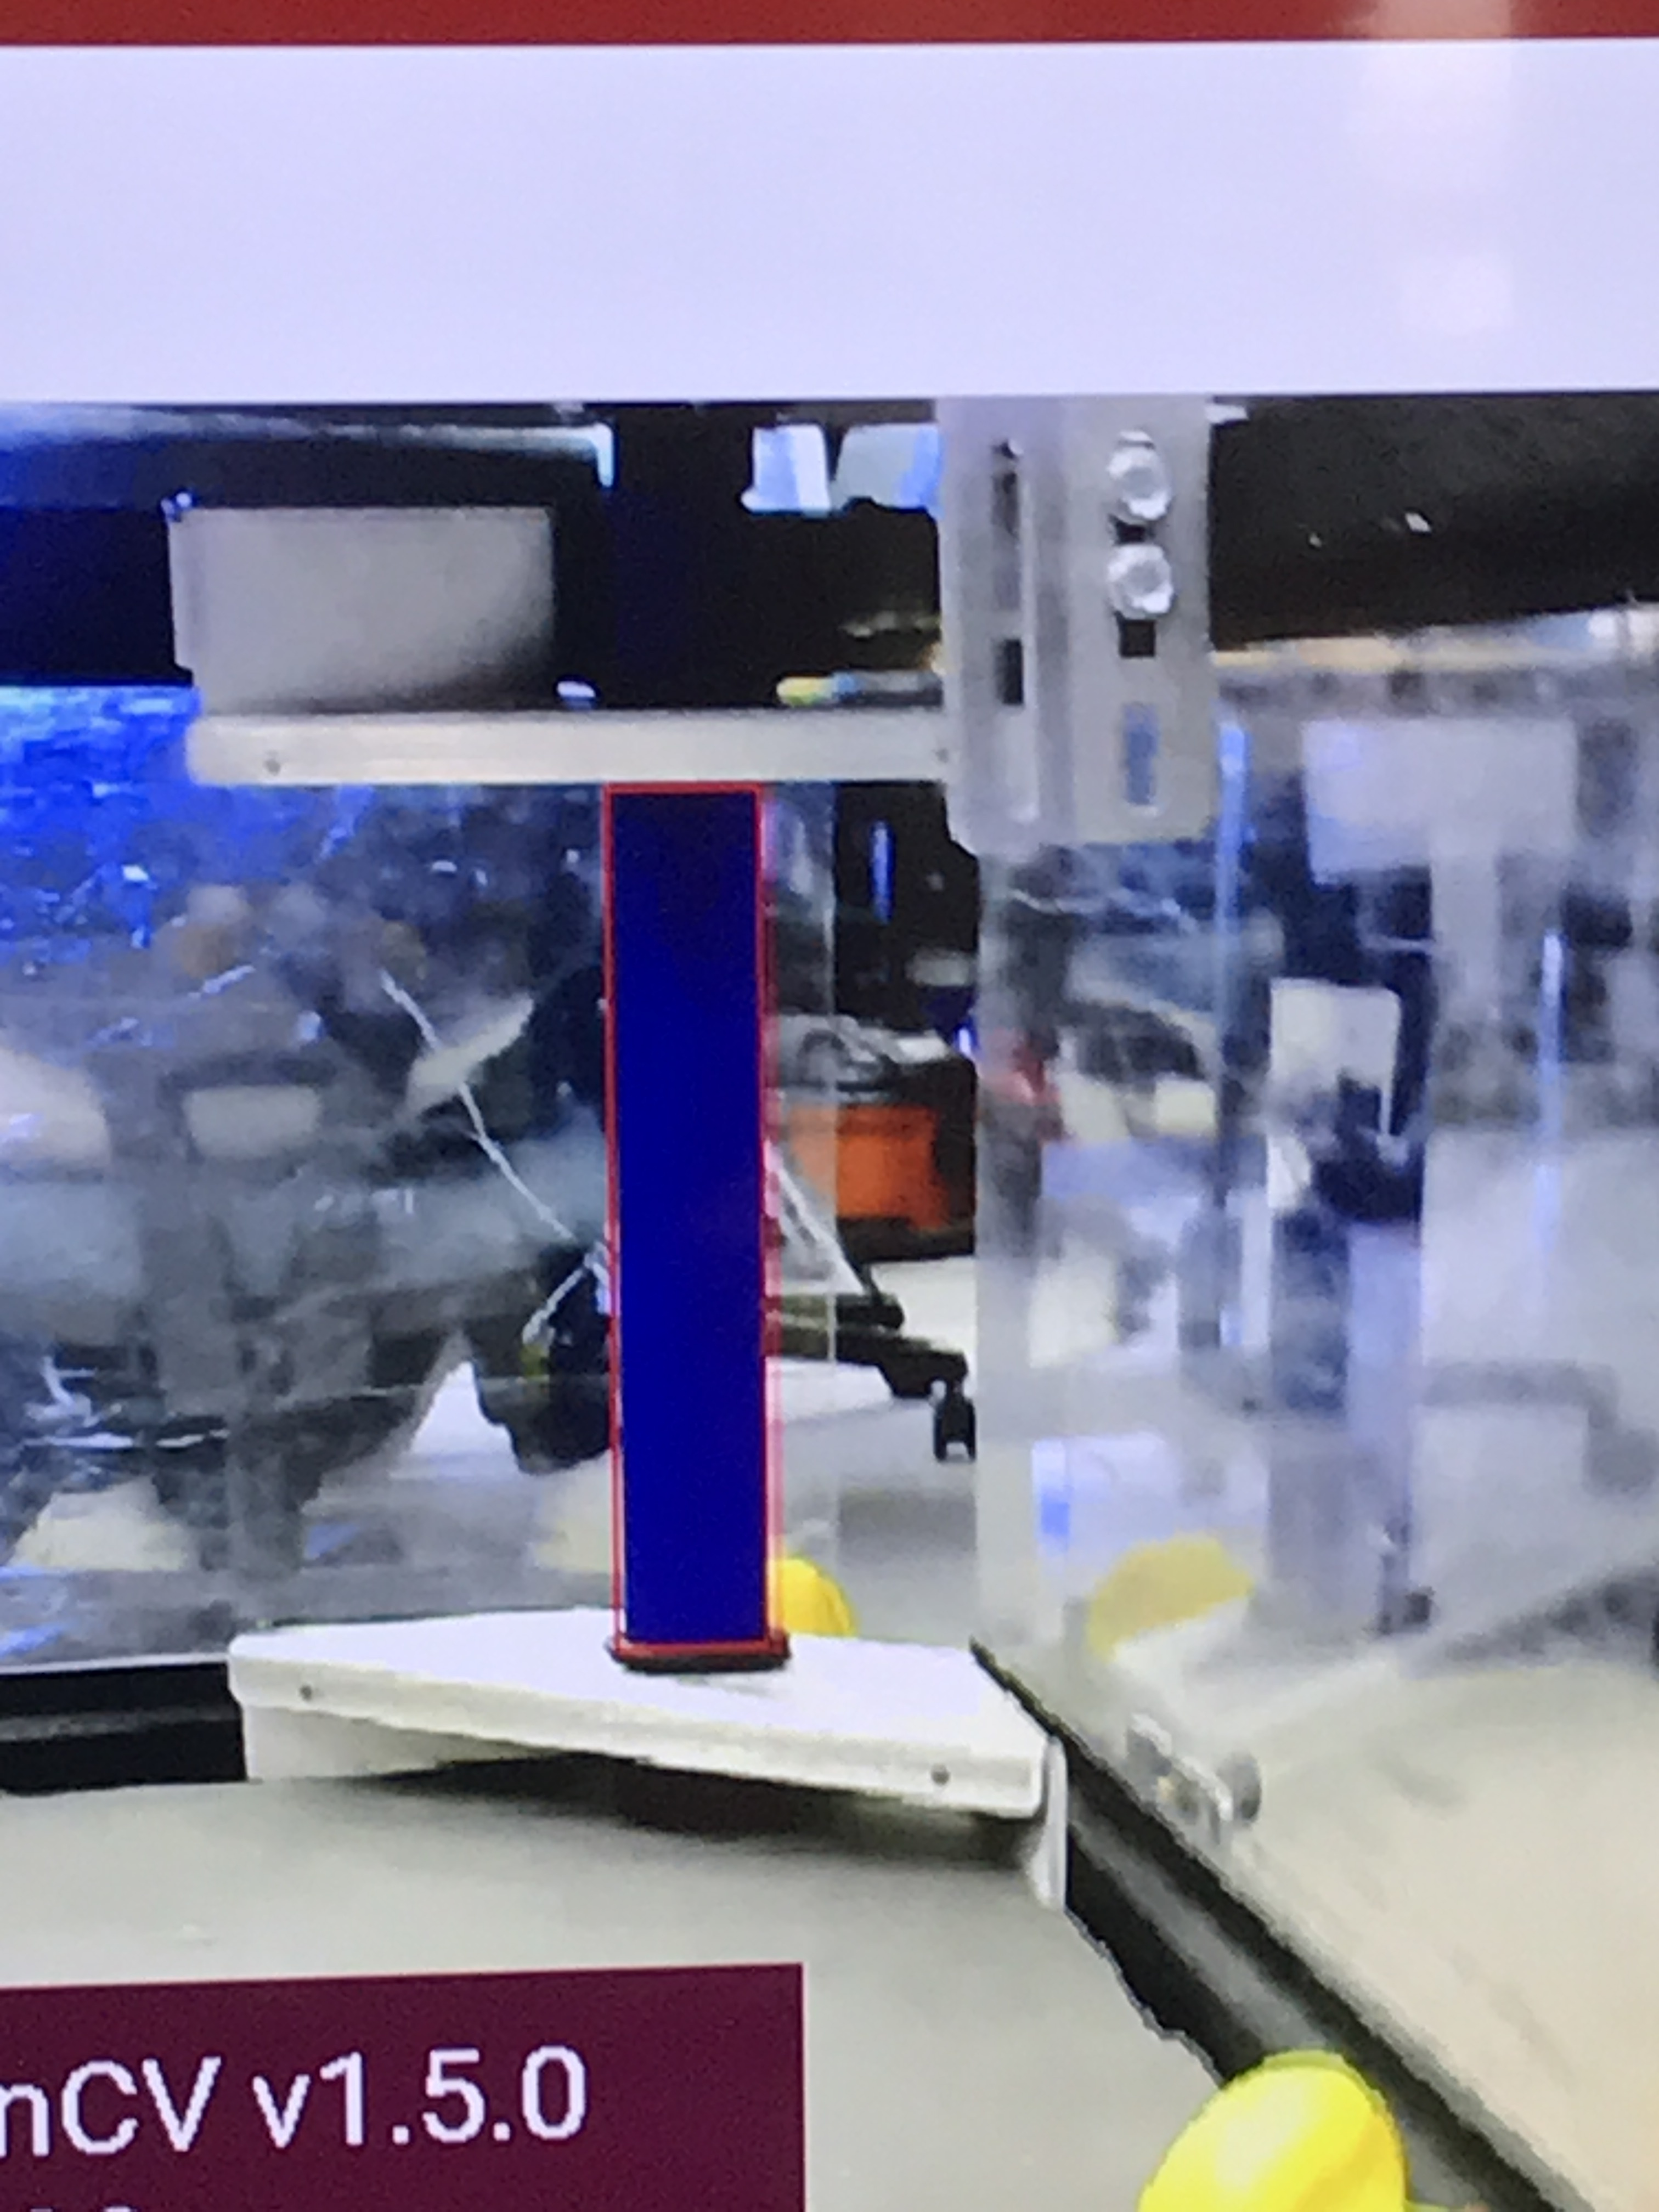
\includegraphics[width=0.95\textwidth]{Meetings/January/01-24-22/IMG_5648 - James Hu.JPG}
  \caption{Our pipeline after filtering the contours to find the largest height to width ratio}
  \label{fig:012422_2}
\end{minipage}
\end{figure}



\whatsnext{
\begin{itemize}
    \item Finish and test the pipeline for the red carousel on the opposite side of the field
\end{itemize} 
}

